%%%%%%%%%%%%%%%%%%%%%%%%%%%%%%%%%%%%%%%%%
% HW Template
% LaTeX Template
% Version 1.0 (19/10/18)
% Modified by
% Erdem TUNA
% Halil TEMURTAŞ 
% Enes TAŞTAN 
%%%%%%%%%%%%%%%%%%%%%%%%%%%%%%%%%%%%%%%%%
%
%----------------------------------------------------------------------------------------
%	PACKAGES AND OTHER DOCUMENT CONFIGURATIONS
%----------------------------------------------------------------------------------------
\documentclass[a4paper,12pt]{article}
%-----packages------
\usepackage[a4paper, total={6.2in, 8.5in}]{geometry}
\usepackage[english]{babel}
\usepackage[utf8x]{inputenc}
\usepackage{amsmath}
\usepackage{graphicx}
\usepackage[colorinlistoftodos]{todonotes}
\usepackage{gensymb} % this could be problem
\usepackage{float}
\usepackage{fancyref}
\usepackage{subcaption}
\usepackage[toc,page]{appendix} %appendix package
\usepackage{xcolor}
\usepackage{listings}
\usepackage{xspace}
\usepackage{amssymb}
\usepackage{nicefrac}
\usepackage{gensymb}
\usepackage{fancyhdr}
\usepackage{blindtext}  % for dummy text, use \blindtext or \BlindText
\usepackage{lipsum}    % for dummy text, use \lipsum[3-56]
\usepackage[final]{pdfpages}  % pdf include
\usepackage{array} %allows more options in tables
\usepackage{pgfplots,pgf,tikz} %coding plots in latex
\usepackage{capt-of} % allows caption outside the figure environment
\usepackage[export]{adjustbox} %more options for adjusting the images
\usepackage{multicol,multirow,slashbox} % allows tables like table1
%\usepackage[hyperfootnotes=false]{hyperref} % clickable references
\usepackage{epstopdf} % useful when matlab is involved
%\usepackage{placeins} % prevents the text after figure to go above figure with \FloatBarrier 
%\usepackage{listingsutf8,mcode} %import .m or any other code file mcode is for matlab highlighting

%-----end of packages

%-----specifications-----
\definecolor{mGreen}{rgb}{0,0.6,0} % for python
\definecolor{mGray}{rgb}{0.5,0.5,0.5}
\definecolor{mPurple}{rgb}{0.58,0,0.82}
\definecolor{mygreen}{RGB}{28,172,0} % color values Red, Green, Blue for matlab
\definecolor{mylilas}{RGB}{170,55,241}

\setcounter{secnumdepth}{5} % how many sectioning levels to assign numbers to
\setcounter{tocdepth}{5}    % how many sectioning levels to show in ToC

\lstdefinestyle{CStyle}{
	commentstyle=\color{mGreen},
	keywordstyle=\color{magenta},
	numberstyle=\tiny\color{mGray},
	stringstyle=\color{mPurple},
	basicstyle=\footnotesize,
	breakatwhitespace=false,         
	breaklines=true,
	frame=single,
	rulecolor=\color{black!40},                 
	captionpos=b,                    
	keepspaces=true,                 
	numbers=left,                    
	numbersep=5pt,                  
	showspaces=false,                
	showstringspaces=false,
	showtabs=false,                  
	tabsize=2,
	language=C
}

\lstset{language=Matlab,%
	%basicstyle=\color{red},
	breaklines=true,%
	frame=single,
	rulecolor=\color{black!40},
	morekeywords={matlab2tikz},
	keywordstyle=\color{blue},%
	morekeywords=[2]{1}, keywordstyle=[2]{\color{black}},
	identifierstyle=\color{black},%
	stringstyle=\color{mylilas},
	commentstyle=\color{mygreen},%
	showstringspaces=false,%without this there will be a symbol in the places where there is a space
	numbers=left,%
	numberstyle={\tiny \color{black}},% size of the numbers
	numbersep=9pt, % this defines how far the numbers are from the text
	emph=[1]{for,end,break},emphstyle=[1]\color{red}, %some words to emphasise
	%emph=[2]{word1,word2}, emphstyle=[2]{style},    
}


\tikzset{
	desicion/.style={
		diamond,
		draw,
		text width=4em,
		text badly centered,
		inner sep=0pt
	},
	block/.style={
		rectangle,
		draw,
		text width=10em,
		text centered,
		rounded corners
	},
	cloud/.style={
		draw,
		ellipse,
		minimum height=2em
	},
	descr/.style={
		fill=white,
		inner sep=2.5pt
	},
	connector/.style={
		-latex,
		font=\scriptsize
	},
	rectangle connector/.style={
		connector,
		to path={(\tikztostart) -- ++(#1,0pt) \tikztonodes |- (\tikztotarget) },
		pos=0.5
	},
	rectangle connector/.default=-2cm,
	straight connector/.style={
		connector,
		to path=--(\tikztotarget) \tikztonodes
	}
}

\tikzset{
	desicion/.style={
		diamond,
		draw,
		text width=4em,
		text badly centered,
		inner sep=0pt
	},
	block/.style={
		rectangle,
		draw,
		text width=10em,
		text centered,
		rounded corners
	},
	cloud/.style={
		draw,
		ellipse,
		minimum height=2em
	},
	descr/.style={
		fill=white,
		inner sep=2.5pt
	},
	connector/.style={
		-latex,
		font=\scriptsize
	},
	rectangle connector/.style={
		connector,
		to path={(\tikztostart) -- ++(#1,0pt) \tikztonodes |- (\tikztotarget) },
		pos=0.5
	},
	rectangle connector/.default=-2cm,
	straight connector/.style={
		connector,
		to path=--(\tikztotarget) \tikztonodes
	}
}
%-----end of specifications-----


%----commands----
\newcommand\nd{\textsuperscript{nd}\xspace}
\newcommand\rd{\textsuperscript{rd}\xspace}
\newcommand\nth{\textsuperscript{th}\xspace} %\th is taken already
\newcommand{\specialcell}[2][c]{ \begin{tabular}[#1]{@{}c@{}}#2\end{tabular}} % for too long table lines

\newcommand{\blankpage}{
	\- \\[9cm]	
	{ \centering \textit{This page intentionally left blank.} \par }
	\- \\[9cm]
}% For Blank Page

\makeatletter
\renewcommand\paragraph{\@startsection{paragraph}{4}{\z@}%
	{-2.5ex\@plus -1ex \@minus -.25ex}%
	{1.25ex \@plus .25ex}%
	{\normalfont\normalsize\bfseries}}
\makeatother
%-----end of commands-----


\pagestyle{fancy}
\fancyhead[LO,LE]{Halil TEMURTAŞ / 2094522   }
\fancyhead[RO,RE]{November 5,2018}
\fancyfoot[RO,RE]{
\includegraphics[width=2.7cm]{eelogo}}

\begin{document}
\begin{center}
	\textbf{\large EE402 Discrete Time Systems \\[0.2cm] MP-2} \\
\end{center}


\begin{enumerate}
	\item 
		\begin{enumerate}
			\item 	$x[k]=9k2^k-4^k+3$ \\
			It is known that one-sided Z-Transform of $x[k]=1$ is $X(z)= \mathcal{Z}\{1\}=\cfrac{1}{1-z^{-1}}$
			using the properties and linearity of z-transform
			\begin{itemize}
				\item $	\mathcal{Z}\{a^{k}x[k]\}=X(z/a)$
				\item $	\mathcal{Z}\{kx[k]\}=-z\frac{d}{dz} X(z)	$
			\end{itemize}
			The z-transform of given function can be found as follows;
			$$	\mathcal{Z}\{a^{k}\}=\frac{1}{1-az^{-1}}$$
			$$	X(z)=-9z\frac{d}{dz}(\frac{1}{1-2z^{-1}})-\frac{1}{1-4z^{-1}}+3\frac{1}{1-z^{-1}}	$$
			$$\boxed{	X(z)=\frac{18z^{-1}}{(1-2z^{-1})^{-2}}-\frac{1}{1-4z^{-1}}+3\frac{1}{1-z^{-1}}	}$$
			\item 	$x[k]=\sum_{h=0}^{k}a^h$ where a is a constant\\
			In this part, we can use, causal shifting property of Z-transform, i.e.,
			\begin{itemize}
				\item $	\mathcal{Z}\{x[k-N]\}=z^{N}X(z)$				
			\end{itemize}
			Thus, the z-transform of given function can be found as follows;
			$$x[k-1]=\sum_{h=0}^{k-1}a^{h-1}$$
			$$	x[k]-x[k-1]=a^k $$	
			$$ 	X(z)-z^{-1}X(z)=\mathcal{Z}\{a^{k}\} $$
			$$ 	X(z)(1-z^{-1})=\mathcal{Z}\{a^{k}\} $$	
			$$ 	X(z)=\frac{\mathcal{Z}\{a^{k}\}}{(1-z^{-1})}  $$
			$$	\mathcal{Z}\{a^{k}\}=\frac{1}{1-az^{-1}}$$
			$$\boxed{ X(z)=\frac{1}{(1-z^{-1})(1-az^{-1})} }$$
			
			\newpage
			
			\item 	$ x[k]=k(k-1)...(k-h+1)a^{k-h}$\\
			
			\begin{itemize}
				\item for $h=0$, $x[k]=a^k$ , $\mathcal{Z}\{ x[k] \}= X_0(z)=\frac{1}{1-az^{-1}}$
				\item for $h=1$, $x[k]=ka^{k-1}$ , $\mathcal{Z}\{ x[k] \}= X_1(z)=a^{-1}(-z\frac{d}{dz})X_0(z) =\frac{z^{-1}}{{(1-az^{-1})}^{2}}$
				\item for $h=2$, $x[k]=k(k-1)a^{k-2}$ , $\mathcal{Z}\{ x[k] \}= X_2(z)=a^{-1}(-z\frac{d}{dz}-1)X_1(z)=\frac{z^{-1}(1+az^{-1})}{{(1+az^{-1})}^{3}}$
				\item ...
			\end{itemize}
			iteratively, it can be observed that 
			
			$$\boxed{	X(z)=\frac{z^{-h}}{{(1-az^{-1})}^{h+1}}h! }$$
			\item 	It can be seen from the given graph at the mini-project that, the function $x[n]$ can be written in terms of ramp functions $r[k]=k$; 
			$$\boxed{ x[k]=r[k-2]-r[k-5]	}$$
			using the linearity and casual time shift properties of z-transform 
			\begin{itemize}
				\item $	\mathcal{Z}\{x[k-N]\}=z^{N}X(z) $
			\end{itemize}
			and complex differentiation theorem , i.e.,
			\begin{itemize}
				\item $	\mathcal{Z}\{kx[k]\}=-z\frac{d}{dz} X(z)	$
			\end{itemize}
			The z-transform of given function can be found as follows;
			$$	X(z)=z^{-2}\frac{z^{-1}}{({1-z^{-1}})^2}-z^{-5}\frac{z^{-1}}{({1-z^{-1}})^2}	$$
			$$\boxed{	X(z)=\frac{z^{-3}(1-z^{-3})}{({1-z^{-1}})^2}	}$$
			
			\item
			$$ X(s)=\frac{1-e^{Ts}}{s}\frac{1}{(s+a)^2}=\frac{1-e^{Ts}}{s}G(s)$$
			$$	x(t)=\mathcal{L}^{-1}\{ (\frac{1-e^{Ts}}{s}) G(s) \}=\mathcal{L}^{-1}\{ (\frac{1}{s}) G(s) \}-\mathcal{L}^{-1}\{ (\frac{e^{Ts}}{s}) G(s) \}	$$
			Lets as assume $\hat{G}(s)=\frac{G(s)}{s}$, 
			$$ x(t)=\hat{g}(t)-\hat{g}(t-T) $$
			$$ \mathcal{Z}\{ x(kT) \}=\mathcal{Z}\{ \hat{g}(kT)-\hat{g}(kT-T)=\mathcal{Z}\{ \hat{g}[k]-\hat{g}[k-1]\}=(1-z^{-1})\hat{G}(z) $$
			$$ 	\hat{G}(z)= \mathcal{Z}\{ \mathcal{L}^{-1} \{ \frac{G(s)}{s}\}\}=\mathcal{Z}\{ \mathcal{L}^{-1} \{ \frac{1}{s(s+a)^2} \}\}$$
			To find inverse Laplace transform, we can use partial fraction expansion for the expression, 		
			$$   \frac{1}{s(s+a)^2}  = \frac{a_1}{s}+\frac{a_2}{s+a}+\frac{a_3}{{(s+a)}^2} $$
			With some calculation, coefficients are found to be, \\
			$$ \boxed{a_1=\frac{1}{a^2}} \ ,\ \boxed{a_2=-\frac{1}{a^2}}\ ,\ \boxed{a_3=-\frac{1}{a}} $$			
			Thus,
			$$  \hat{g}(t)  = a_1 +a_2 e^{-at}+ a_3te^{-t} $$
			$$	\hat{g}(t)  = \frac{1}{a^2} -\frac{1}{a^2} e^{-at}-\frac{1}{a}te^{-t} $$	 
			$$ 	\hat{G}(z)= \mathcal{Z}\{ \frac{1}{a^2} -\frac{1}{a^2} e^{-akT}-\frac{1}{a}kTe^{-kT}  \} $$
			$$ 	\hat{G}(z)= \frac{1}{a^2} \frac{1}{1-z^{-1}} - \frac{1}{a^2} \frac{1}{1-e^{-aT}z^{-1}} - \frac{1}{a} \frac{Te^{-aT}z^{-1}}{{(1-e^{-aT}z^{-1})}^2}	$$
			$$	X(z)=(1-z^{-1})(\frac{1}{a^2} \frac{1}{1-z^{-1}} - \frac{1}{a^2} \frac{1}{1-e^{-aT}z^{-1}} - \frac{1}{a} \frac{Te^{-aT}z^{-1}}{{(1-e^{-aT}z^{-1})}^2}	)		$$ 
			$$\boxed{	X(z)=(\frac{1}{a^2} - \frac{1}{a^2} \frac{(1-z^{-1})}{1-e^{-aT}z^{-1}} - \frac{1}{a} \frac{(1-z^{-1})(Te^{-aT}z^{-1})}{{(1-e^{-aT}z^{-1})}^2}	)		}$$ 	
		\end{enumerate}
	
	
	\item $$ X(z)=\frac{z^{-1}}{(1-z^{-1}){(1+1.3z^{-1}+0.4z^{-2})}^2}$$
		$$ X(z)=\frac{z^{4}}{(z-1){(z^2+1.3+0.4z^2)}^2} $$
				
		\begin{enumerate}
			\item Using partial fraction expansion,
			$$ \frac{X(z)}{z}=\frac{a_1}{z-1}+\frac{a_2}{{(z+0.5)}^2}+\frac{a_3}{z+0.5}+\frac{a_4}{{(z+0.8)}^2}+\frac{a_5}{z+0.8} $$
			$$	a_1=lim_{z \to 1 } \frac{X(z)(z-1)}{z} = \frac{100}{729}	$$
			$$	a_2=lim_{z \to -0.5 } \frac{X(z){(z+0.5)}^2}{z} = \frac{100}{729}	$$
			$$	a_3=lim_{z \to -0.5 } \frac{X(z)(z+0.5)}{z} = \frac{-100}{9}	$$
			$$	a_4=lim_{z \to -0.8 } \frac{X(z){(z+0.8)}^2}{z} = \frac{-320}{81}	$$
			$$	a_5=lim_{z \to -0.8 } \frac{X(z)(z+0.8)}{z} = \frac{8000}{729}	$$
			
			Thus, $x[k]$ becomes
			
			$$\boxed { x[k]=\frac{100}{729}- \frac{50}{27}k{(-0.5)}^k- \frac{100}{9}{(-0.5)}^k- \frac{320}{81}k{(-0.8)}^k+ \frac{8000}{729}{(-0.8)}^k	 }$$
			
			Matlab code simulating the result can be found at Appendix A, at lines 46-54.
			\item Matlab code simulating the result can be found at Appendix A, at lines 1-45.
			\item Matlab code simulating the result can be found at Appendix A, at lines 56-71.
			\item Matlab code simulating the result can be found at Appendix A, at lines 72-80.
			\item Matlab code simulating the result can be found at Appendix A, at lines 81-126. The resulting $x[k]s$ can be seen at \textit{Figure~\ref{fig:method}}.
				\begin{figure}[H]
					\center
					\setlength{\unitlength}{\textwidth} 
					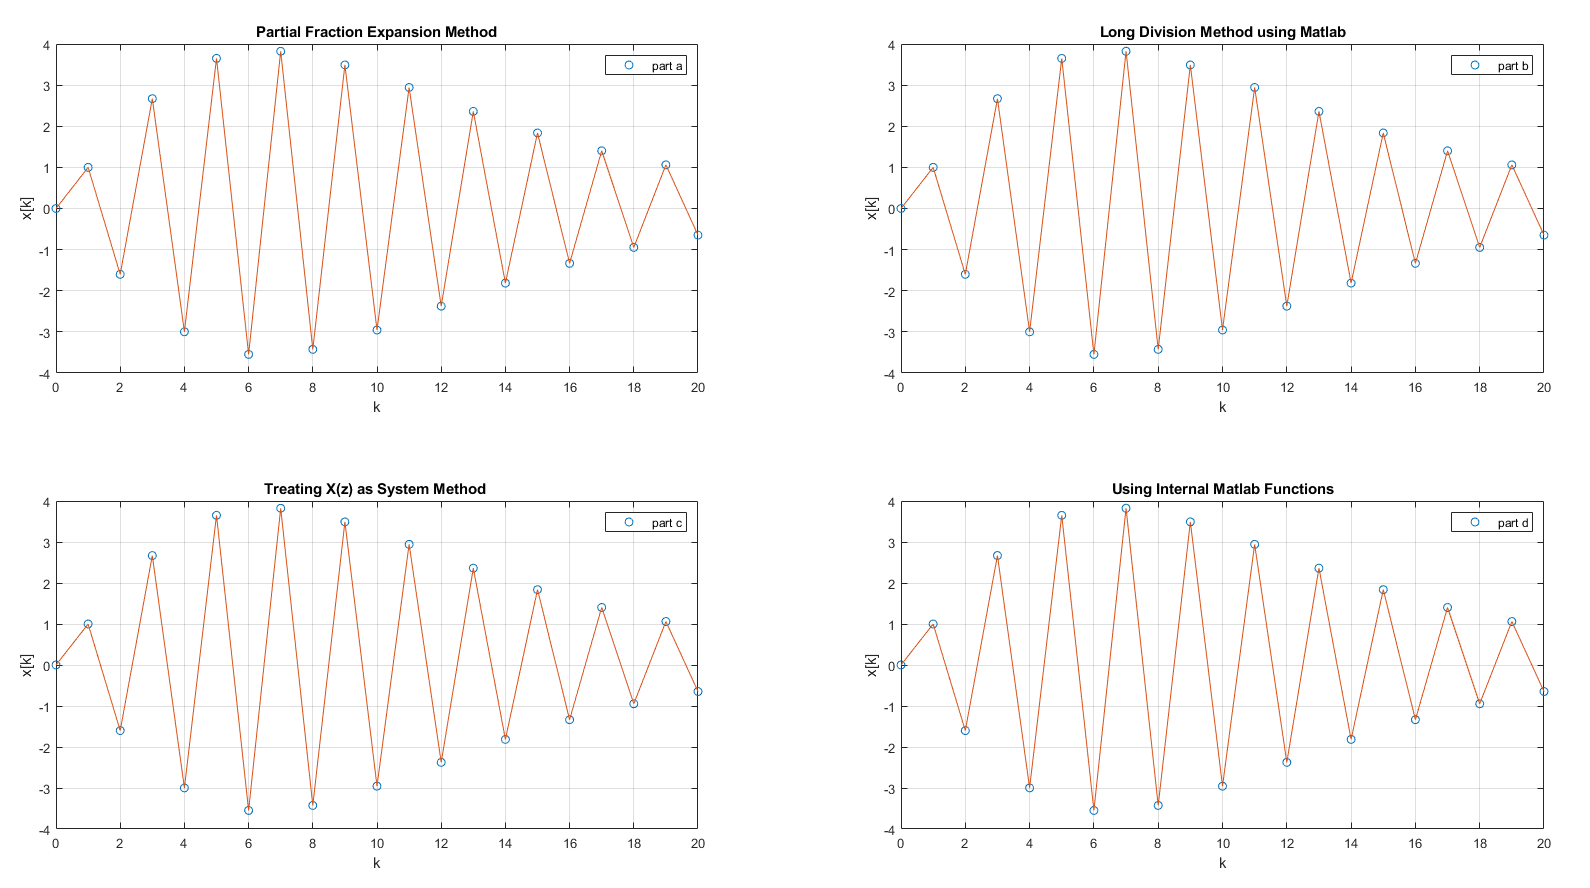
\includegraphics[width=1.0\unitlength]{2e6}
					\caption{\label{fig:method}$x[k]$ plots using different methodologies }
				\end{figure}
		\end{enumerate}
	\item $ y[k]-7y[k-1]+12y[k-2]=x[k]$ , $y[k]=0$ for $k<0$ and $x[k]=52^k+k$, $x[k]=0$ for $k<0$ 
		
		\begin{enumerate}
			\item Assume $x[k]=0$ to find homogeneous solution, it is known that, $y_h[k]$ will be in the form $A^k$.
			$$	A^k-7A^{k-1}+12A^{k-2}=0	$$
			$$	A^{k-2}\left(\ (A-4)(A-3) \right)=0$$
			Thus, it can be observed that, $y_h[k]$ will be in the form $a_14^k+a_23^k$.
			
			To find the the $y_p[k]$, assume it to be in a form close to $x[n]$,i.e., in a form of $b_12^k+b_2k+b_3$. Coefficients can be found by inserting it into the original equation.
			
			$$	b_12^k+b_2k+b_3-7[b_12^{k-1}+b_2(k-1)+b_3]+12[b_12^{k-2}+b_2(k-2)+b_3]=52^k+k	$$
			
			by some arrangement in the equation, coefficients can be found as 
			$$	\boxed{b_1=10} \ , \ \boxed{b_2=\frac{1}{6}} \ , \ \boxed{b_3=\frac{17}{36}}	$$
			
			Thus, $y[n]$ will be in the form $a_14^k+a_23^k+102^k+\frac{1}{6}k+\frac{17}{36} $, to find the unknown coefficients, original equation can be iterated starting from $k=0$.
			
			$$	y[0]=7y[-1]-12y[-2]+x[0]=0-0+5=a_1+a_2+10+\frac{17}{36}$$ 
			$$	y[1]=7y[0]-12y[-1]+x[1]=35-0+11=4a_1+3a_2+20+\frac{1}{6}+\frac{17}{36}$$
			
			handling the algebraic equations, unknown coefficient can be found to be as  
			$$	\boxed{a_1=\frac{376}{9}} \ , \ \boxed{a_2=\frac{-189}{4}} 	$$
			
			$$\boxed{	y[k]=\frac{376}{9}4^k-\frac{189}{4}3^k+102^k+\frac{1}{6}k+\frac{17}{36}	}$$
	
			Matlab code simulating the result can be found at Appendix B, at lines 1-12.			
			
			\item The difference equation can be transferred the z-domain in the following form,
				$$	Y(z) \left[ 1-7z^{-1}+12z^{-2} \right]=X(z)	$$
				$$	H(z)=\frac{Y(z)}{X(z)}=\frac{1}{1-7z^{-1}+12z^{-2}} $$
				with $$ X(z)=5\frac{1}{1-2z^{-1}} + \frac{z^{-1}}{{(1-z^{-1})}^{2}}$$ 
				$Y(z)$ can be found as, \\[1cm]				
				\begin{equation}
					\begin{split} 
				Y(z) & =\cfrac{z^{-1}}{{(1-2z^{-1})}^2(1-7z^{-1}+12z^{-2})}+\cfrac{5}{(1-2z^{-1})(1-7z^{-1}+12z^{-2})} \\
				 & =\frac{z^3}{(z-3)(z-4)(z-1)^2}+\frac{5z^3}{(z-3)(z-4)(z-2)} \end{split} 				\end{equation}				
				using partial fraction expansion 
				$$ Y(z)= \left[ \frac{a_1}{z-3}+\frac{a_2}{z-4}+\frac{a_3}{{(z-1)}^2}+\frac{a_4}{z-1} \right] + \left[ \frac{b_1}{z-3} +\frac{b_2}{z-4} + \frac{b_3}{z-2} \right]  $$
				with some calculation coefficients can be found to be 
				$$ \ \boxed{a_1=-9/4}	\ , \ \boxed{a_2=16/9}	\ , \ \boxed{a_3=1/6}	\ , \ \boxed{a_4=17/36}	\ $$ $$ \ \boxed{b_1=-45} \ , \ \boxed{b_2=40}	\ , \ \boxed{b_3=10}	\ $$	
				Then, $y[k]$ becomes
				$$\boxed{	y[k]=\frac{-189}{4}3^k+\frac{376}{9}4^k+102^k+\frac{1}{6}k+\frac{17}{36}	}$$
			Matlab code simulating the result can be found at Appendix B, at lines 13-24.
			\item Matlab code simulating the result can be found at Appendix B, at lines 25-34.
			\item Matlab code simulating the result can be found at Appendix B, at lines 36-68.The resulting $x[k]s$ can be seen at \textit{Figure~\ref{fig:method2}}.
			
				\begin{figure}[H]
					\center
					\setlength{\unitlength}{\textwidth} 
					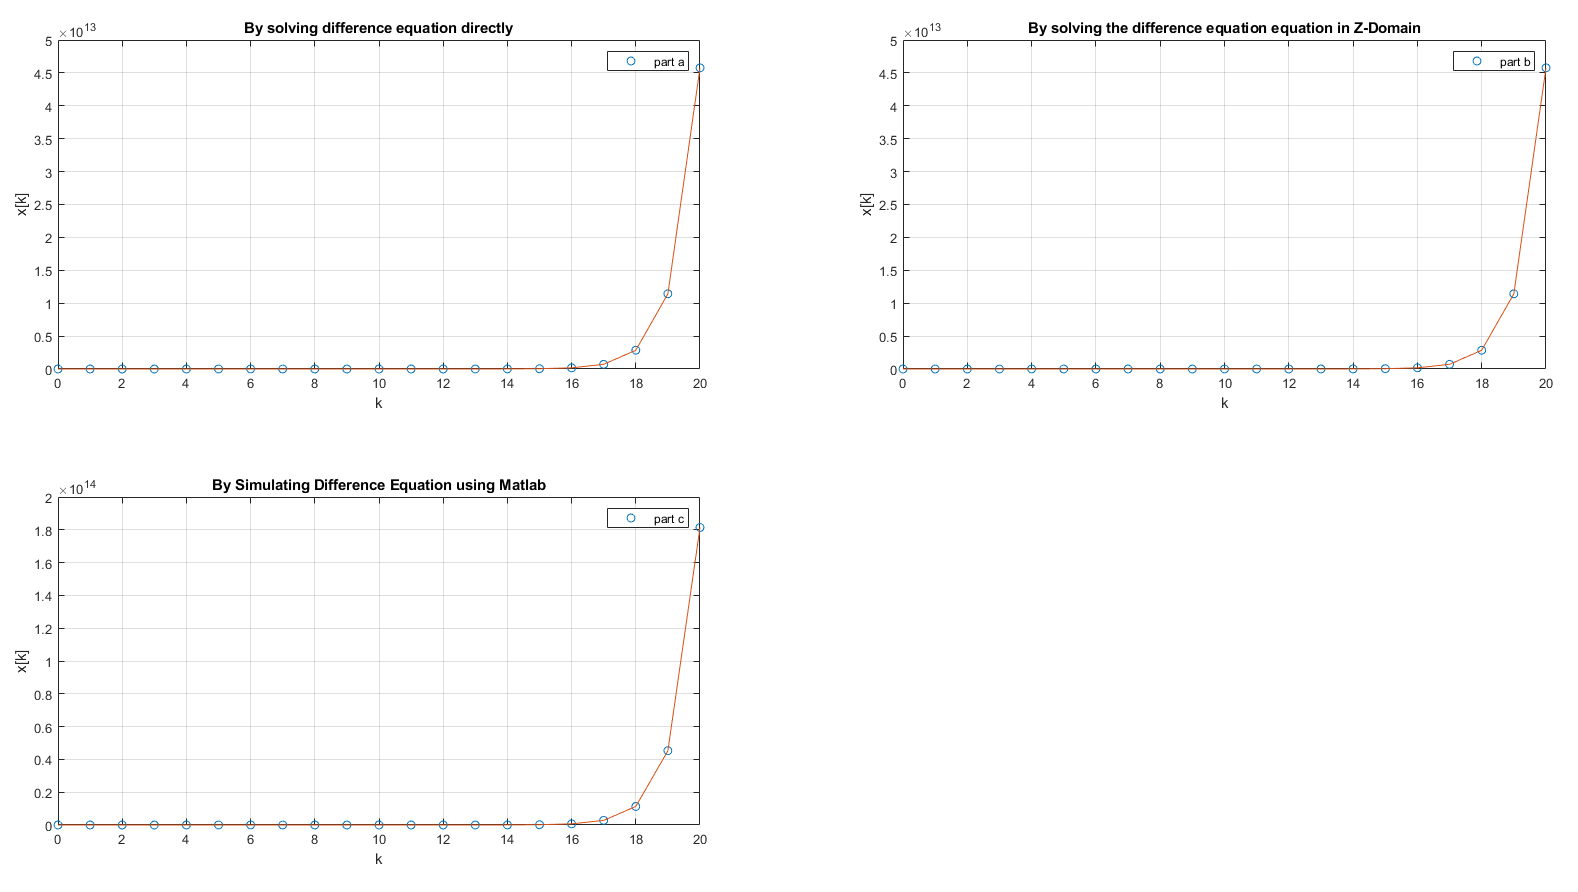
\includegraphics[width=1.0\unitlength]{3d2}
					\caption{\label{fig:method2}$y[k]$ plots using different methodologies }
				\end{figure}
		
		
		\end{enumerate}
	\item $$	G(z)=\frac{4-0.02z^{-1}+0.3z^{-2}+0.02z^{-3}}{2-6z^{-1}+2z^{-2}-z^{-3}+z^{-4}}=\frac{Y(z)}{X(z)}	$$
		Assume a middle variable $H(z)$	
		$$ G_1(z)=\frac{H(z)}{X(z)}$$
		$$ G_2(z)=\frac{Y(Z)}{H(z)} $$
		with
		$$ G_1(z)=4-0.02z^{-1}+0.3z^{-2}+0.02z^{-3} $$
		$$ G_2(z)= 2-6z^{-1}+2z^{-2}-z^{-3}+z^{-4} $$
		from there, it can be observed that if the inverse z-transform is performed on both equations,
		$$\boxed{	x[k]=2h[k]-6h[k-1]+2h[k-2]-8h[k-3]+0.2h[k-4] }$$
		$$\boxed{	y[k]=4h[k]-0.02h[k-1]+0.3h[k-2]+0.02h[k-3] }$$
		
		The resulting block diagram constructed at Simulink can be seen at \textit{Figure~\ref{fig:simu}}
		\begin{figure}[H]
			\center
			\setlength{\unitlength}{\textwidth} 
			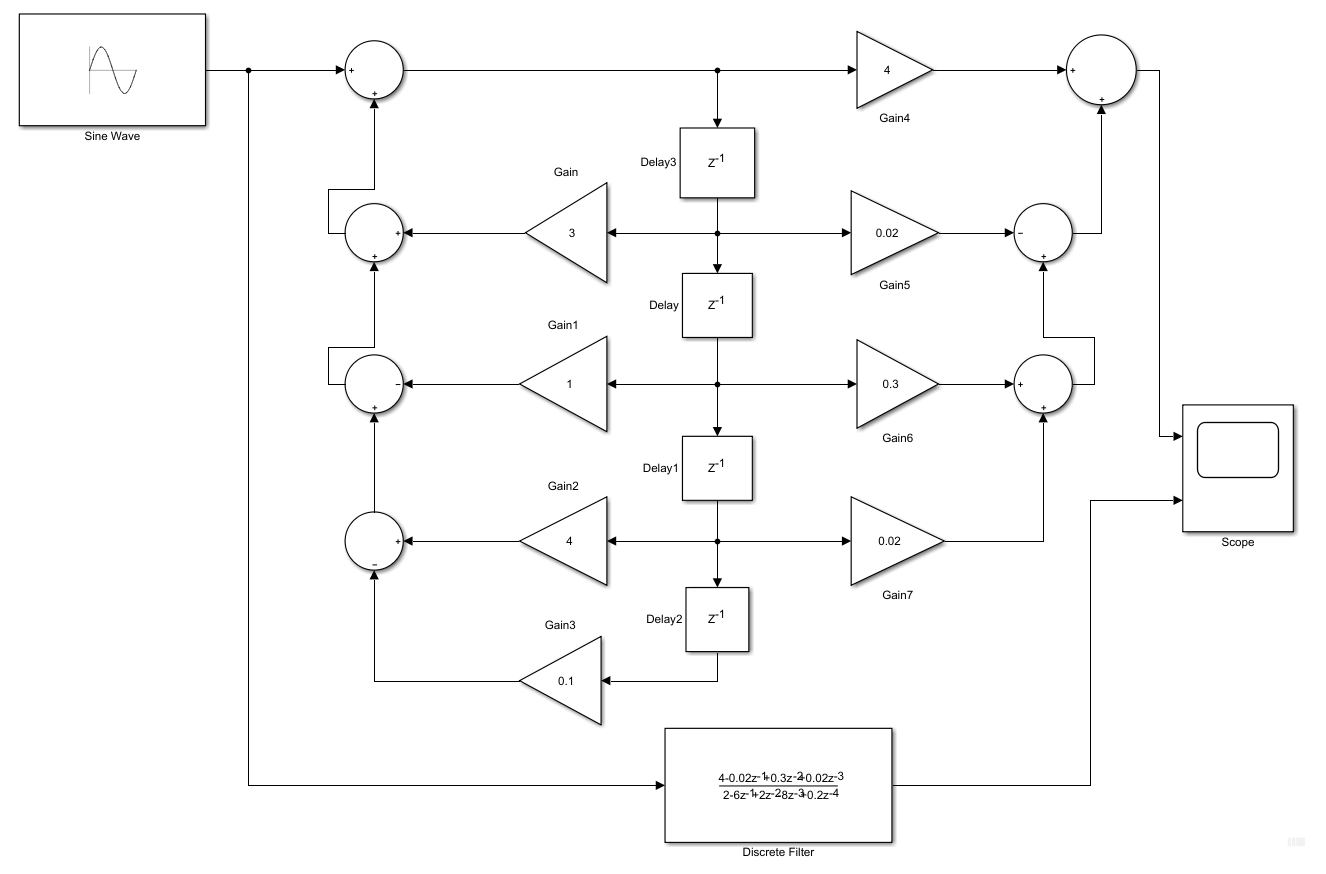
\includegraphics[width=1.0\unitlength]{model3}
			\caption{\label{fig:simmu} Block Diagram of system given at question 4  }
		\end{figure}
				
			
		Differences in the simulation results can be observed form \textit{Figure~\ref{fig:simu1}\ to \ref{fig:simu2}}.
	\begin{figure}[H]
			\center
			\setlength{\unitlength}{\textwidth} 
  		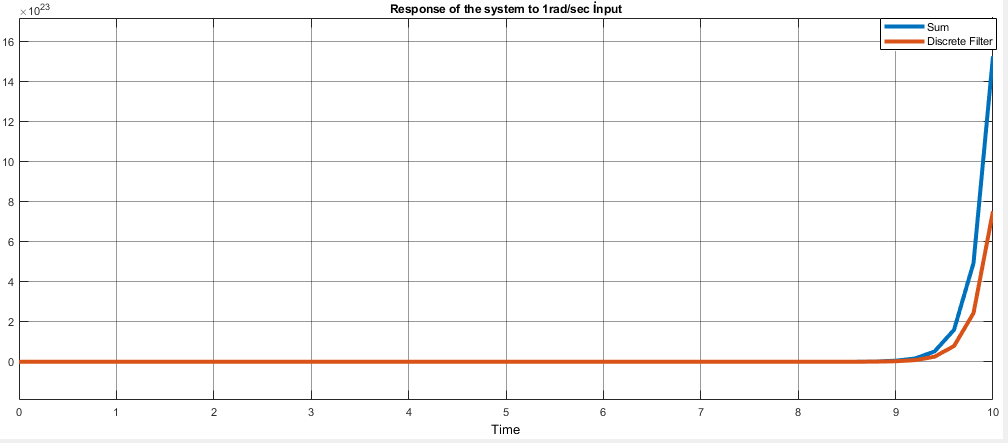
\includegraphics[width=1.0\unitlength]{415}
  		\caption{\label{fig:simu1}Response of the system to 1rad/sec Input }
  	\end{figure}
	
	\begin{figure}[H]
			\center
			\setlength{\unitlength}{\textwidth} 
		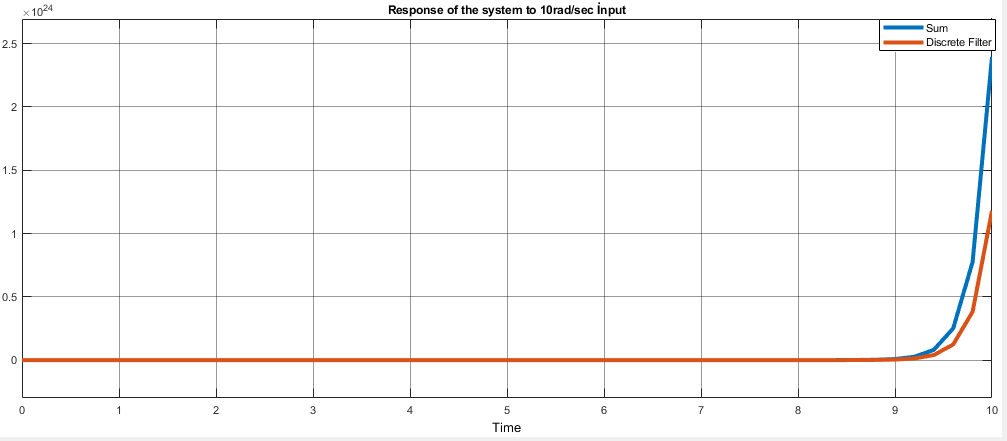
\includegraphics[width=1.0\unitlength]{435}
  		\caption{\label{fig:simu2}Response of the system to 10rad/sec Input}
	\end{figure}
	
	\begin{figure}[H]
			\center
			\setlength{\unitlength}{\textwidth} 
  		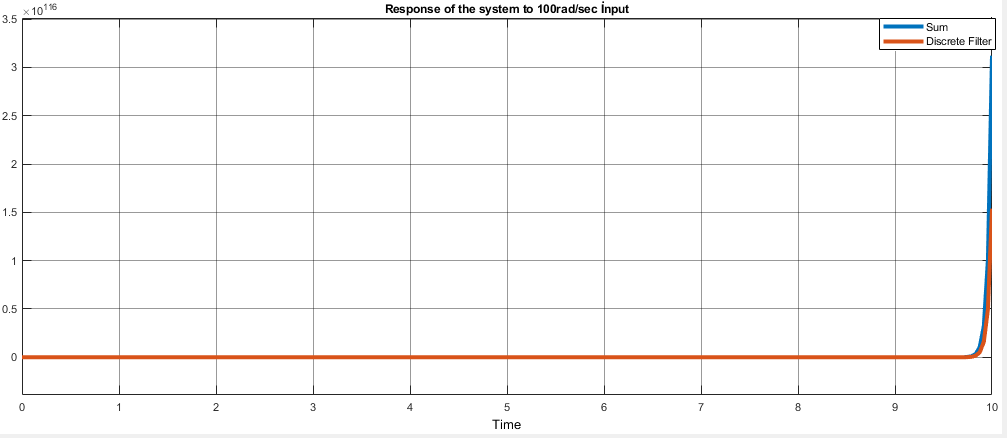
\includegraphics[width=1.0\unitlength]{455}
  		\caption{\label{fig:simu3}Response of the system to 5jjj0rad/sec Input }
	\end{figure}
		
	\begin{figure}[H]
			\center
			\setlength{\unitlength}{\textwidth} 
		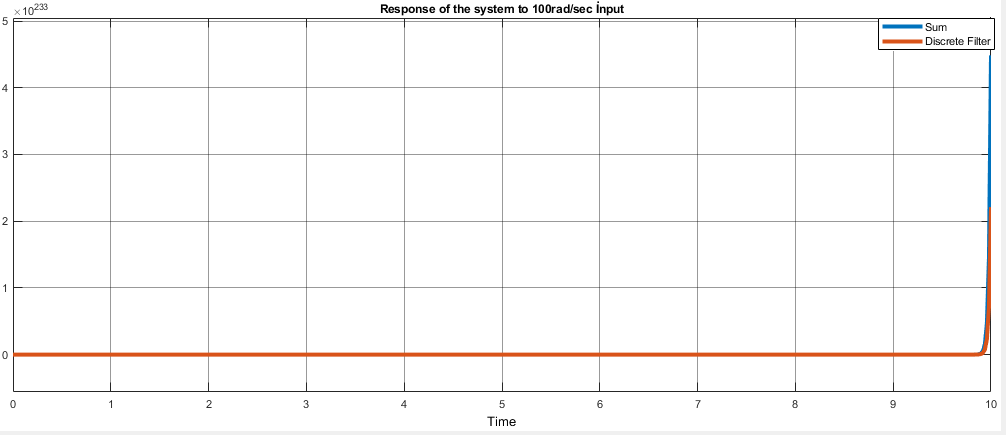
\includegraphics[width=1.0\unitlength]{475}
  		\caption{\label{fig:simu4}Response of the system to 100rad/sec Input}
	\end{figure}
	
	As the frequency is increased, the results became more similar. The internal block is not functioning well enough. However, our design is functioning better than our expectations. 	
	
\end{enumerate}
	
		\newpage
\begin{appendices}
	\section{Source Code For Question 2}
		\lstinputlisting[language=Matlab]{q2.m} \-\\[1cm]

		\lstinputlisting[language=Matlab]{mydelta.m} \-\\[1cm]
		\newpage
	\section{Source Code For Question 3}
		\lstinputlisting[language=Matlab]{q3.m} \-\\[1cm]
%	\section{Source Code For Question 4}
%		\lstinputlisting[language=Matlab]{q4.m} \-\\[1cm]
%				\lstinputlisting[language=Matlab,firstline=33, lastline=34]{q13.m} \-\\[1cm]
\end{appendices}
				


\end{document}

%----samples------
%\begin{itemize}
%\item Item
%\item Item
%\end{itemize}

%\begin{figure}[H]
%\center
%\setlength{\unitlength}{\textwidth} 
%\includegraphics[width=0.7\unitlength]{images/logo1}
%\caption{\label{fig:logo}Logo }
%\end{figure}

%\begin{figure}[H]
%	\setlength{\unitlength}{\textwidth} 
%	\centering
%	\begin{subfigure}{.5\textwidth}
%  		\centering
%  		\includegraphics[width=0.48\unitlength]{images/logo1}
%  		\caption{\label{fig:logo1}Logo1 }
%	\end{subfigure}%
%	\begin{subfigure}{.5\textwidth}
%  		\centering
%		\includegraphics[width=0.48\unitlength]{images/logo2}
%  		\caption{\label{fig:logo2}Logo2}
%	\end{subfigure}
%\caption{\label{fig:calisandegree} Small Logos   }
%\end{figure}
	
%\begin{table}[H]
%  \centering
% 
%    \begin{tabular}{c|c|c}
%       $$A$$ & $$B$$ & $$C$$ \\ \hline
%       1 & 2 & 3  \\ \hline
%       2 & 3 & 4  \\ \hline
%       3 & 4 & 5  \\ \hline
%       4 & 5 & 6  
%      
%  \end{tabular}
%  \caption{table}
%  \label{tab:table}
%\end{table}
	
%\begin{table}[H]
%  \centering
% 
%    \begin{tabular}{c|c|c}
%       \backslashbox{$A$}{$a$} & $$\specialcell{ Average deviation \\ after subtracting out the  \\ frequency error }$$ & $$C$$ \\ \hline
%       \multirow{2}{*}{1} & 2 & 3  \\ \cline{2-3}
%        & 3 & 4  \\ \hline
%       3 & \multicolumn{2}{c}{4}  \\ \hline
%       4 & 5 & 6  
%      
%  \end{tabular}
%  \caption{table}
%  \label{tab:table}
%\end{table}
%-----end of samples-----